\section{Fertigungsunterlagen}

Die CAD-Baugruppe, sämtliche modellierte Einzelteile, die Übersichtszeichnung und Einzelteilzeichnungen sind in im mitabgegebenen ZIP-Ordner enthalten.

\section{Zahnräder, Zahnriemenräder und Zahnriemen}

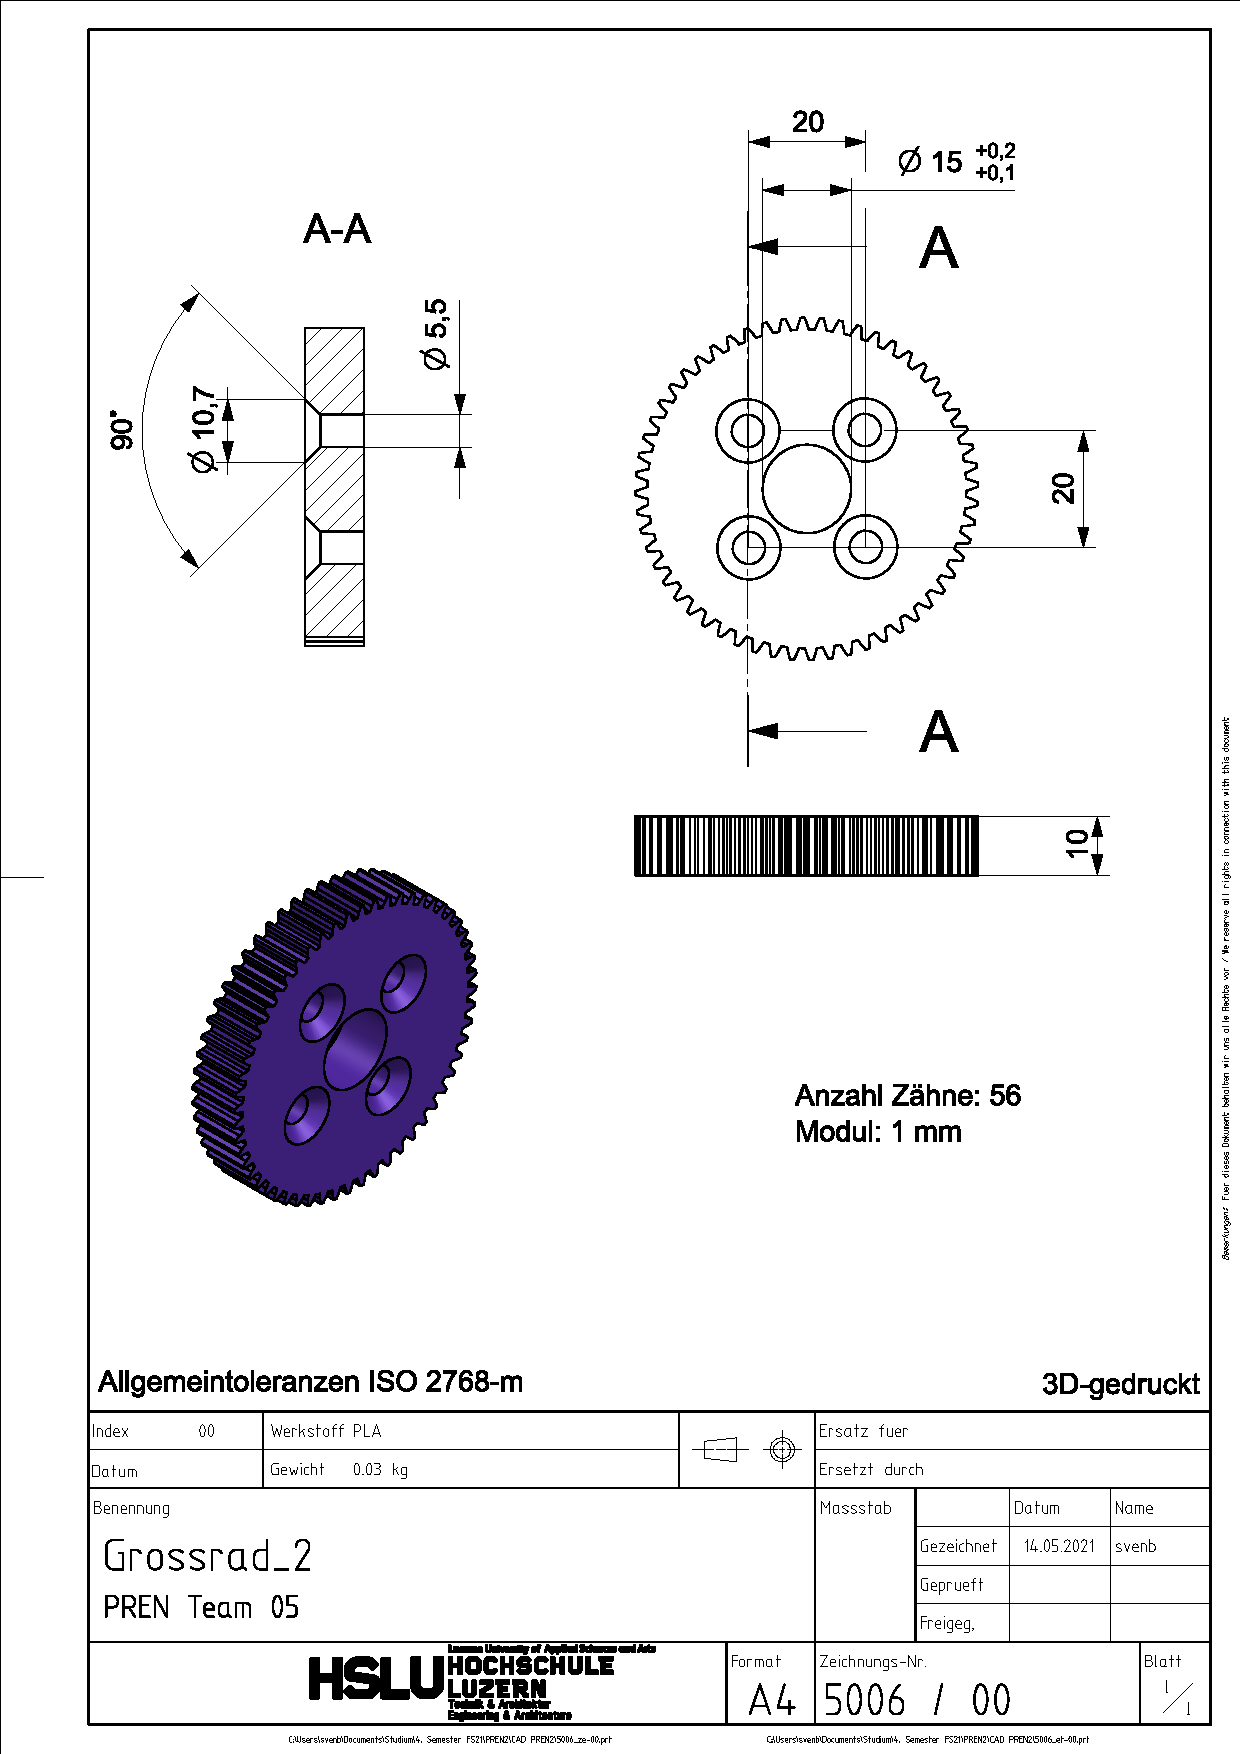
\includepdf[
  pages={1-},
  scale=0.8,
  pagecommand={\pagestyle{fancy}}
]{assets/Fertigungsunterlagen/5006_ze-00.pdf}

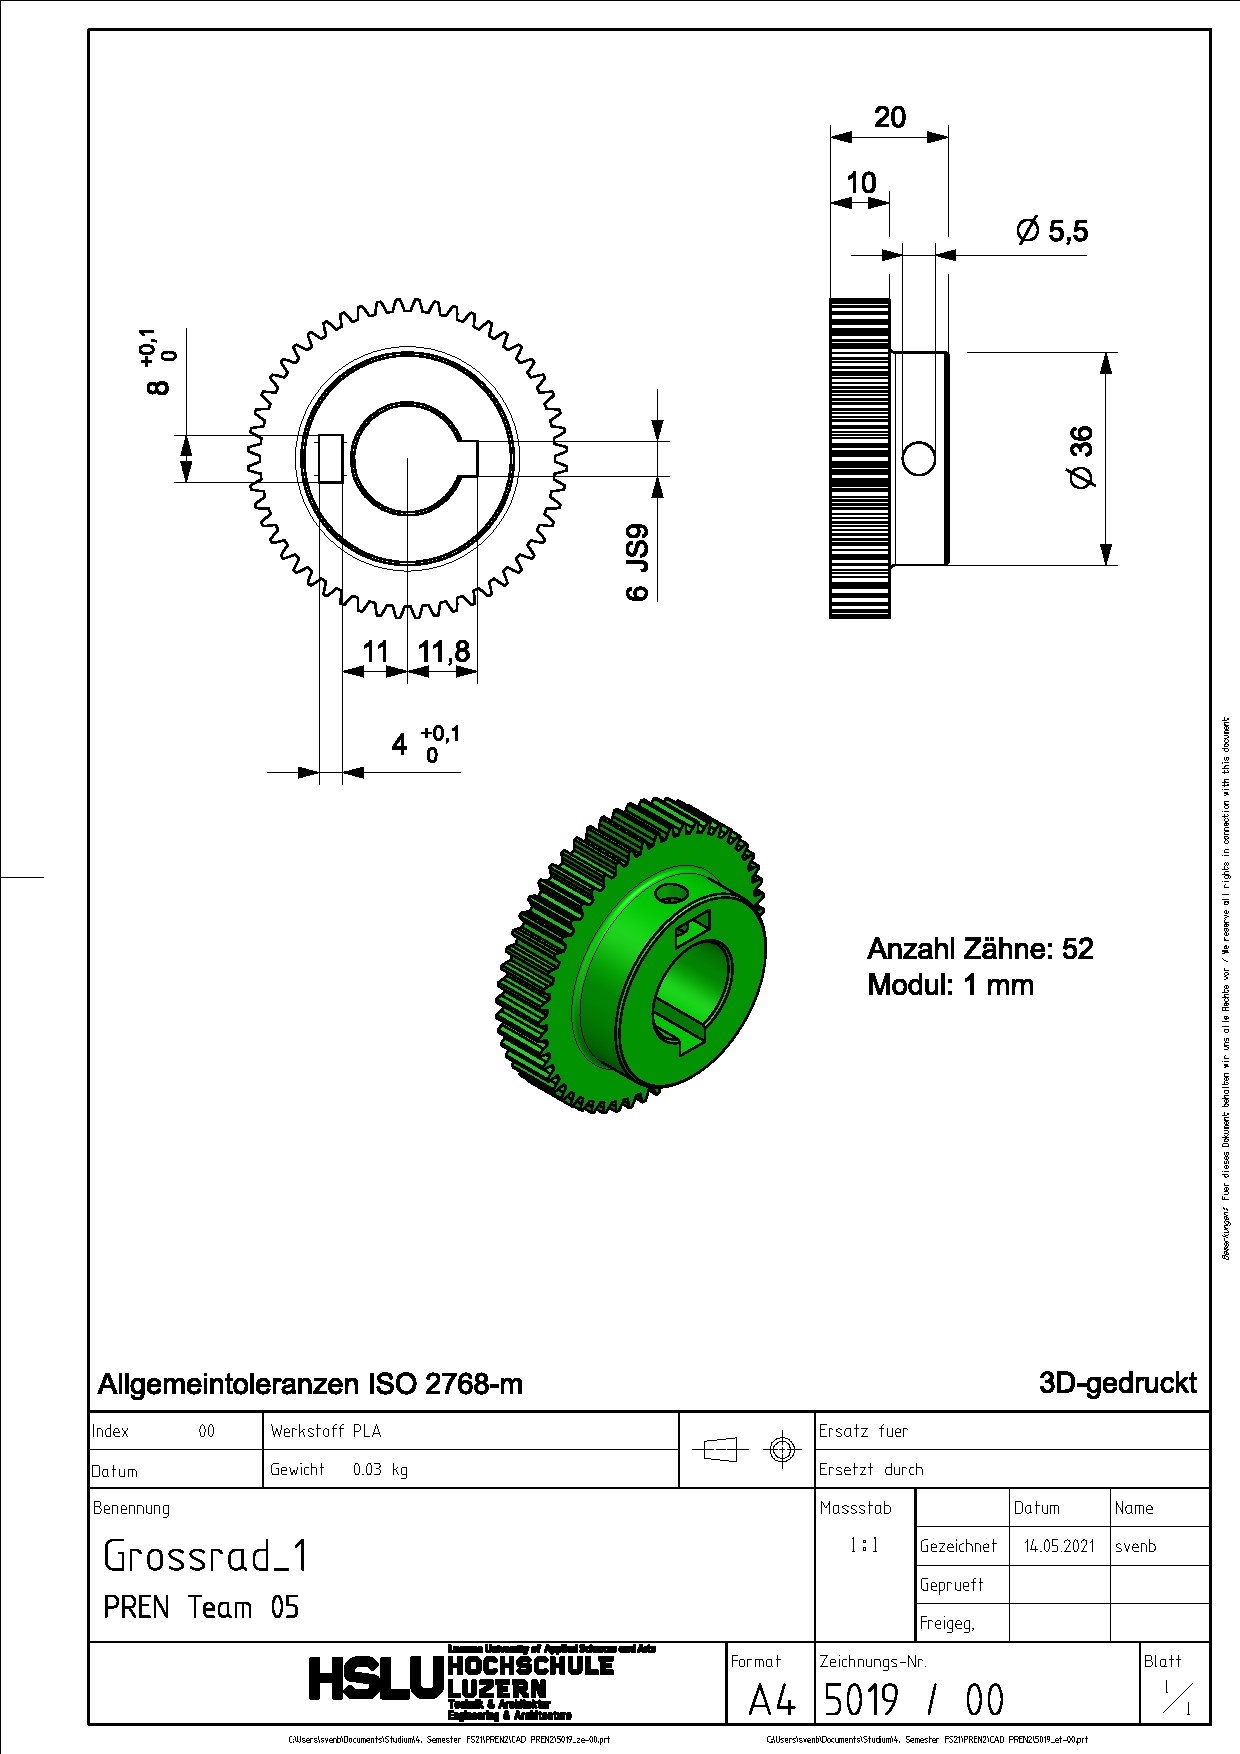
\includepdf[
  pages={1-},
  scale=0.8,
  pagecommand={\pagestyle{fancy}}
]{assets/Fertigungsunterlagen/5019_ze-00.pdf}

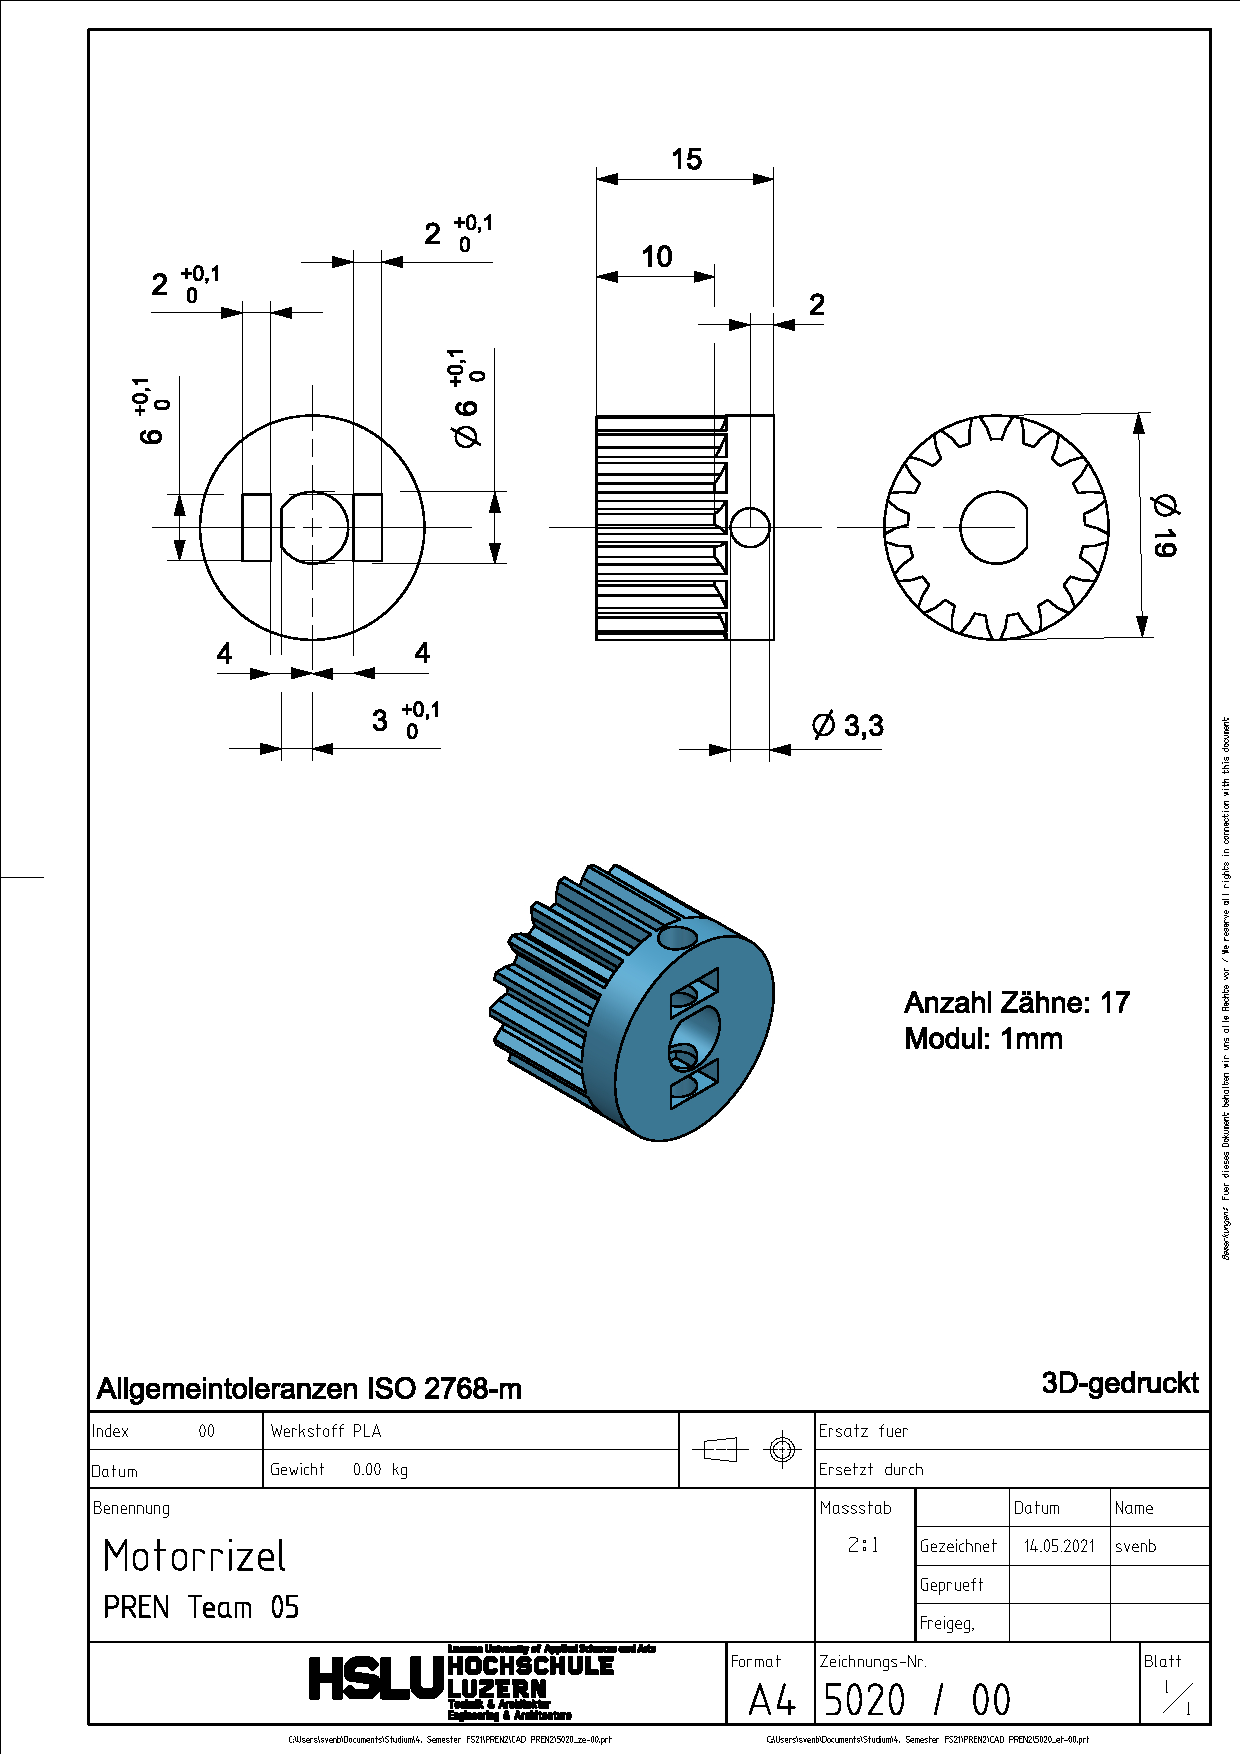
\includepdf[
  pages={1-},
  scale=0.8,
  pagecommand={\pagestyle{fancy}}
]{assets/Fertigungsunterlagen/5020_ze-00.pdf}

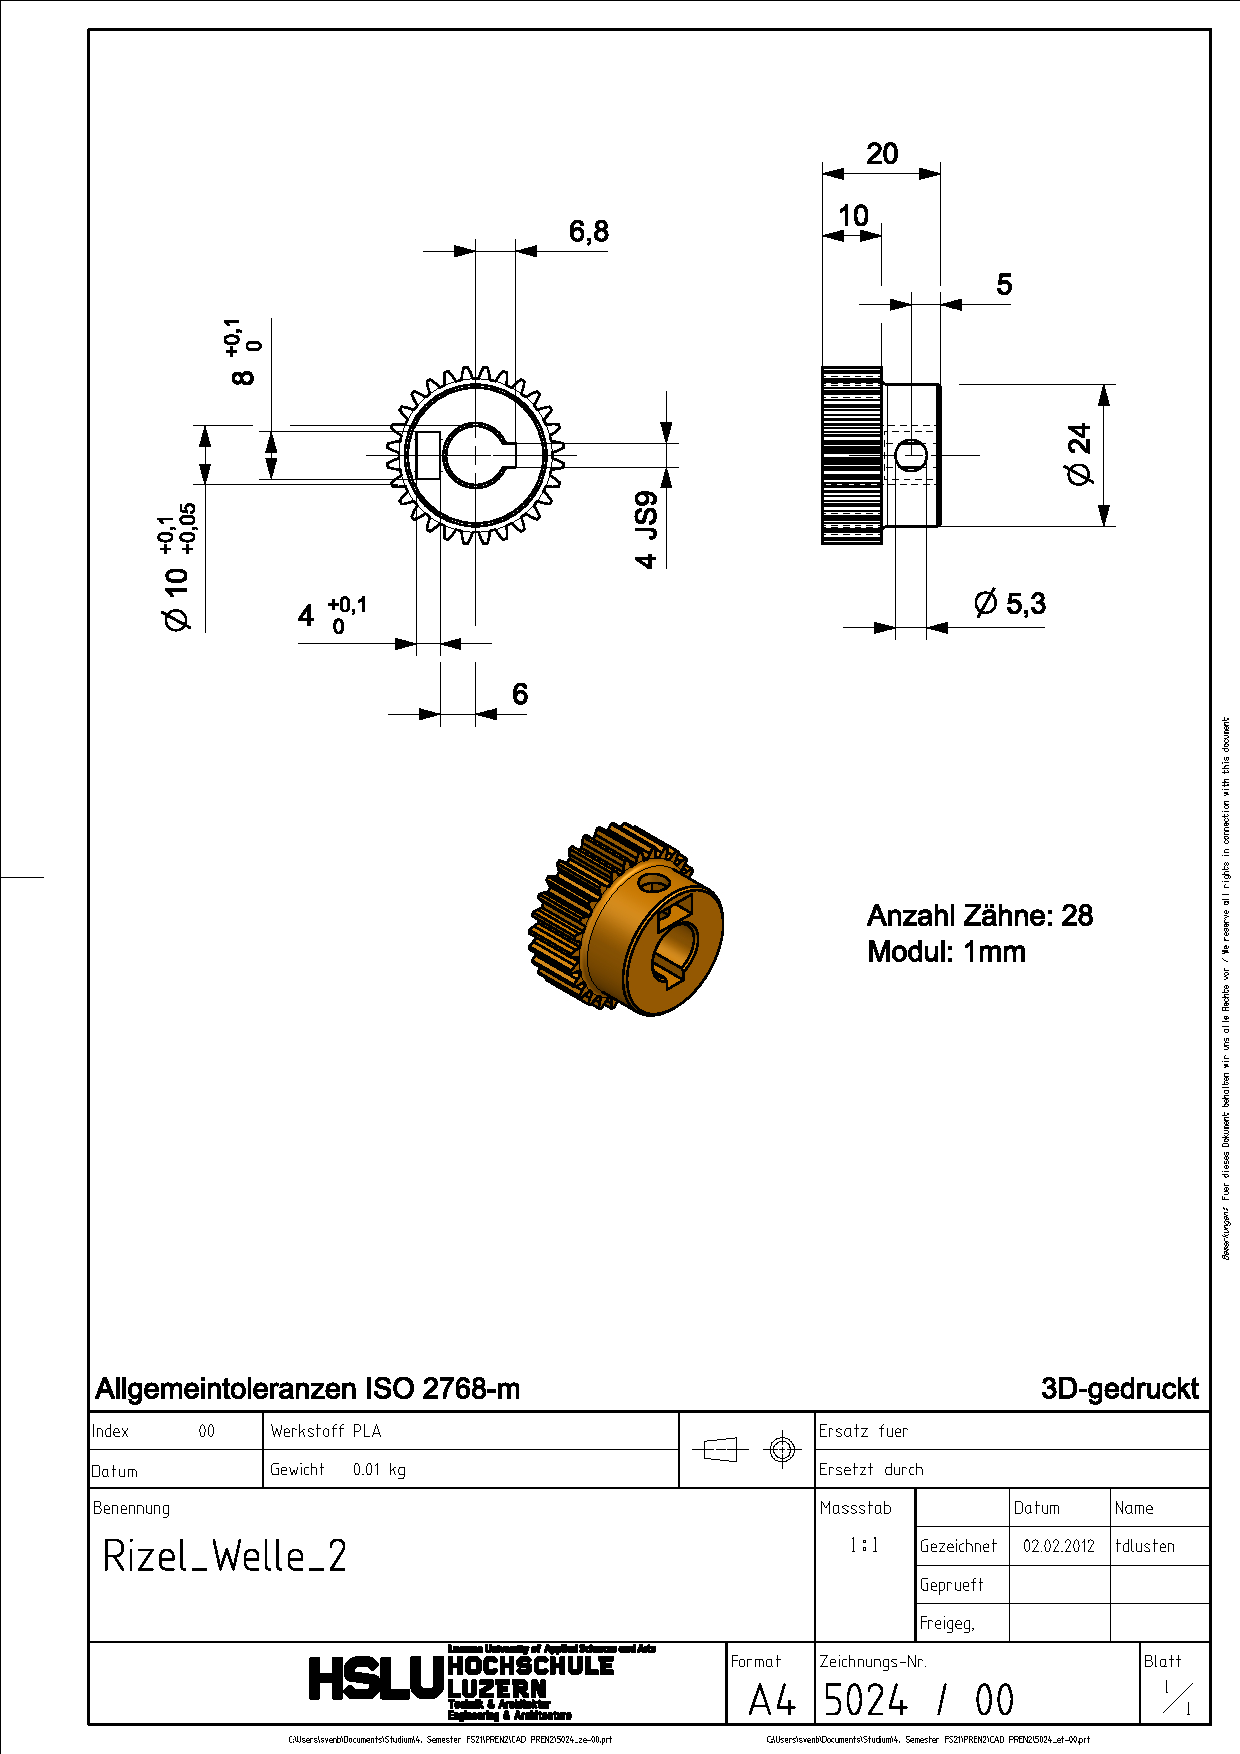
\includepdf[
  pages={1-},
  scale=0.8,
  pagecommand={\pagestyle{fancy}}
]{assets/Fertigungsunterlagen/5024_ze-00.pdf}

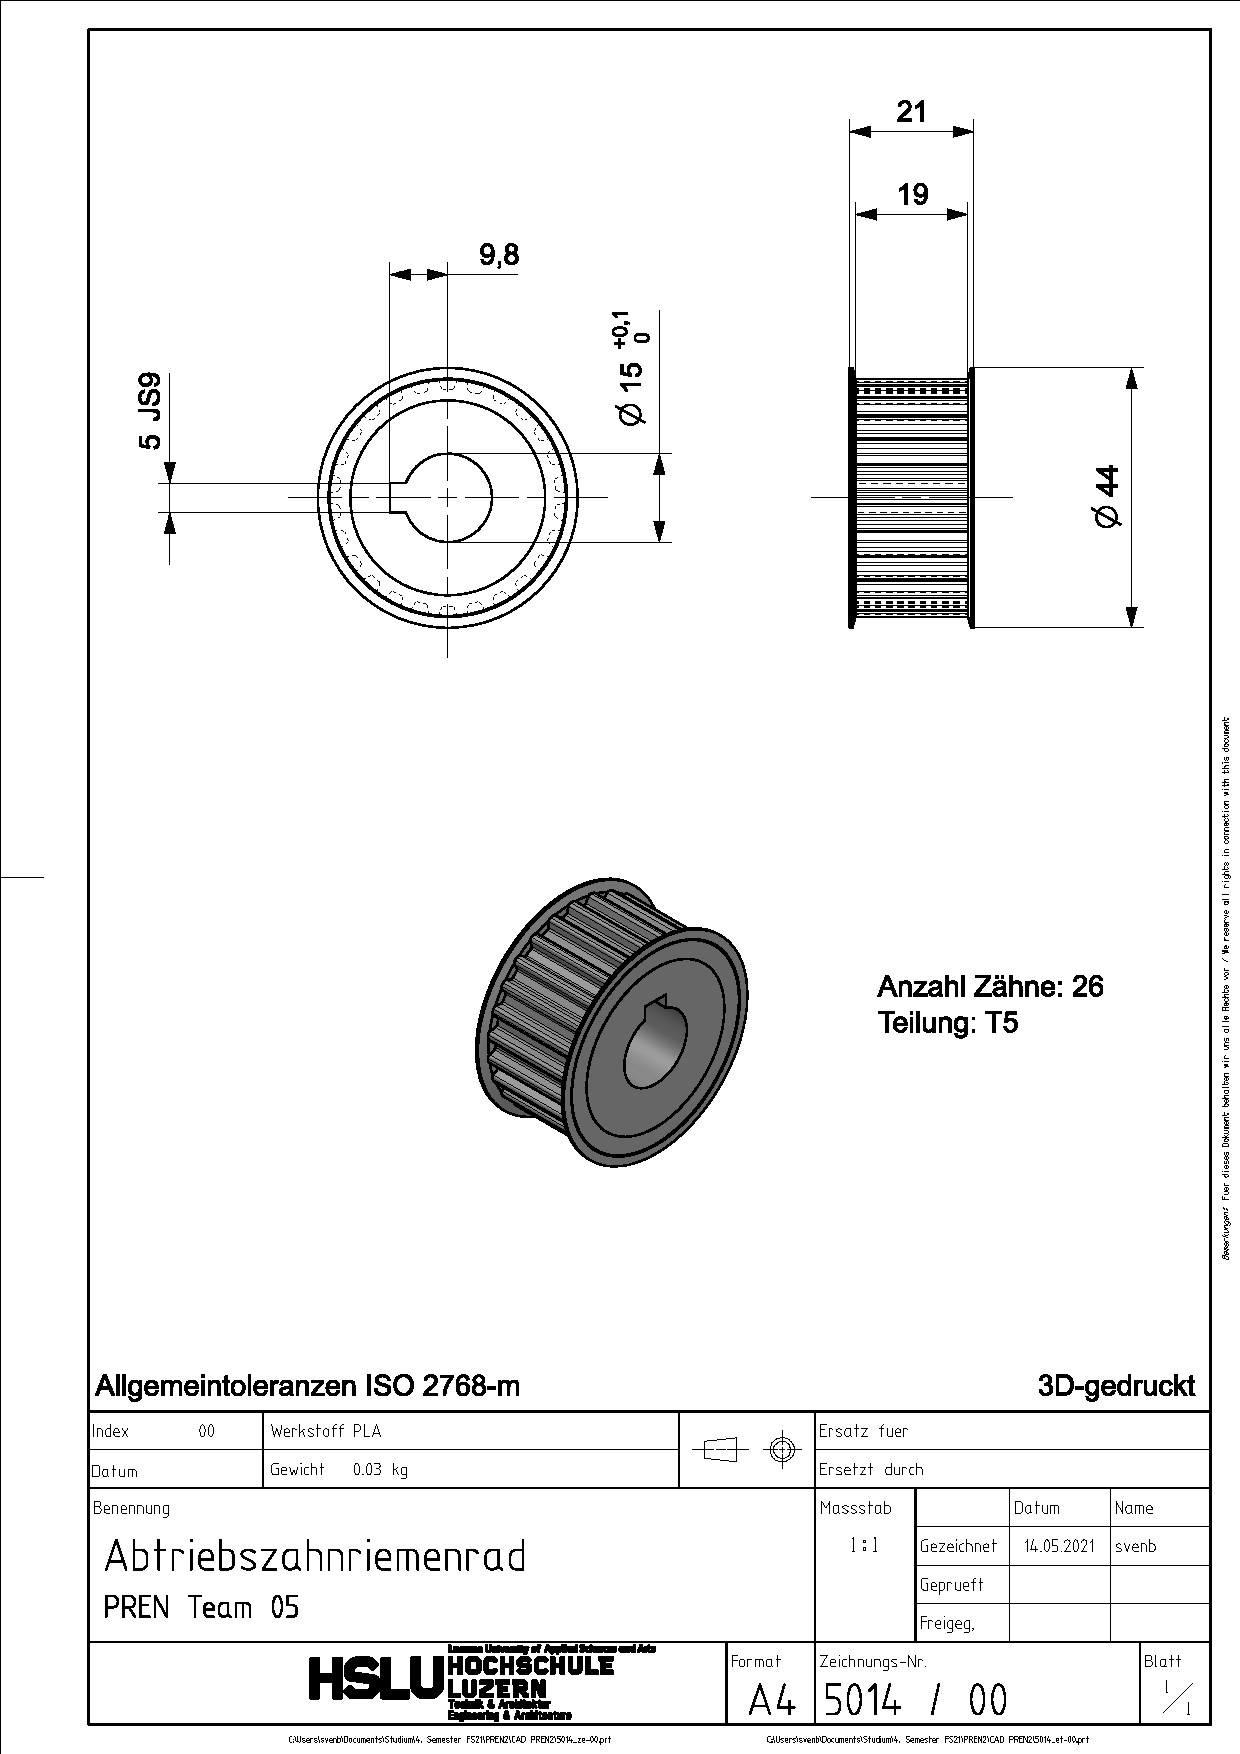
\includepdf[
  pages={1-},
  scale=0.8,
  pagecommand={\pagestyle{fancy}}
]{assets/Fertigungsunterlagen/5014_ze-00.pdf}

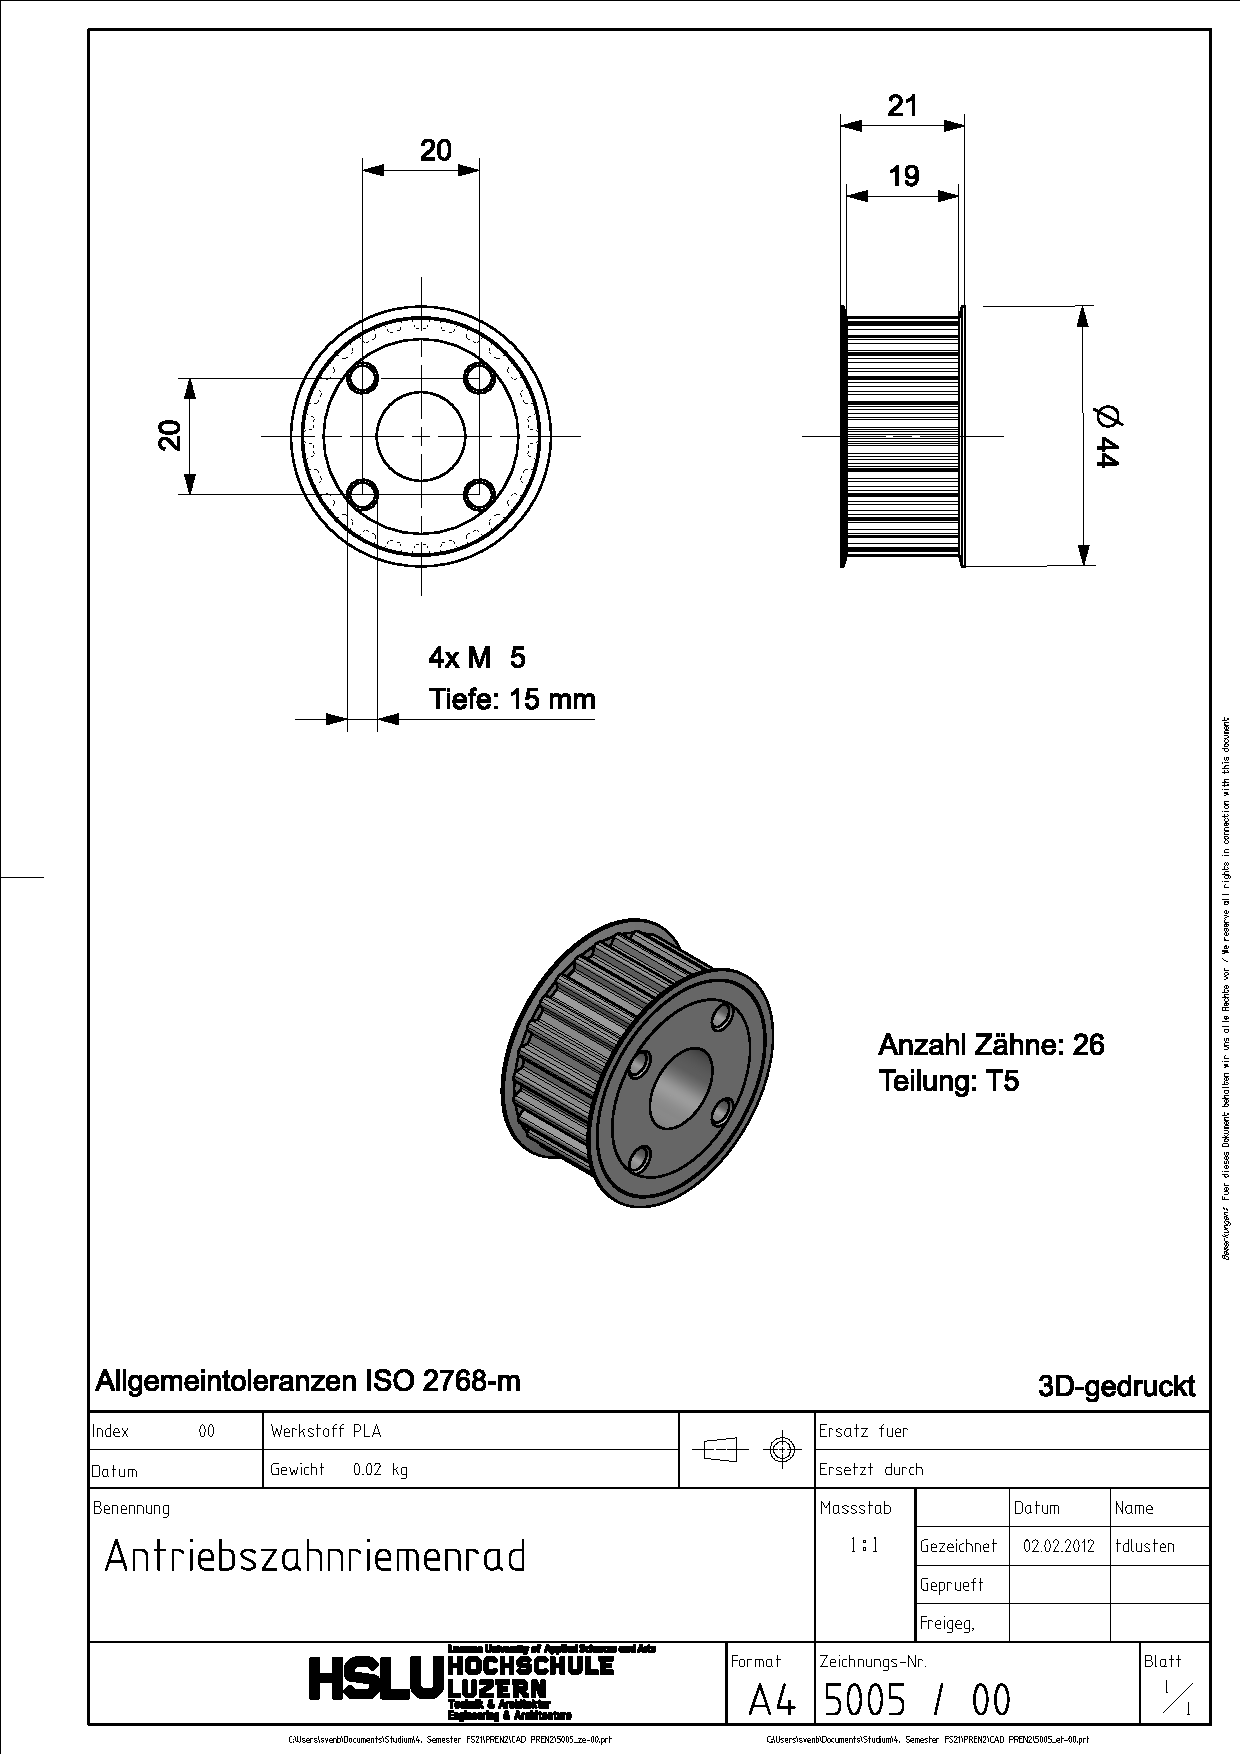
\includepdf[
  pages={1-},
  scale=0.8,
  pagecommand={\pagestyle{fancy}}
]{assets/Fertigungsunterlagen/5005_ze-00.pdf}

\begin{figure}[H]
  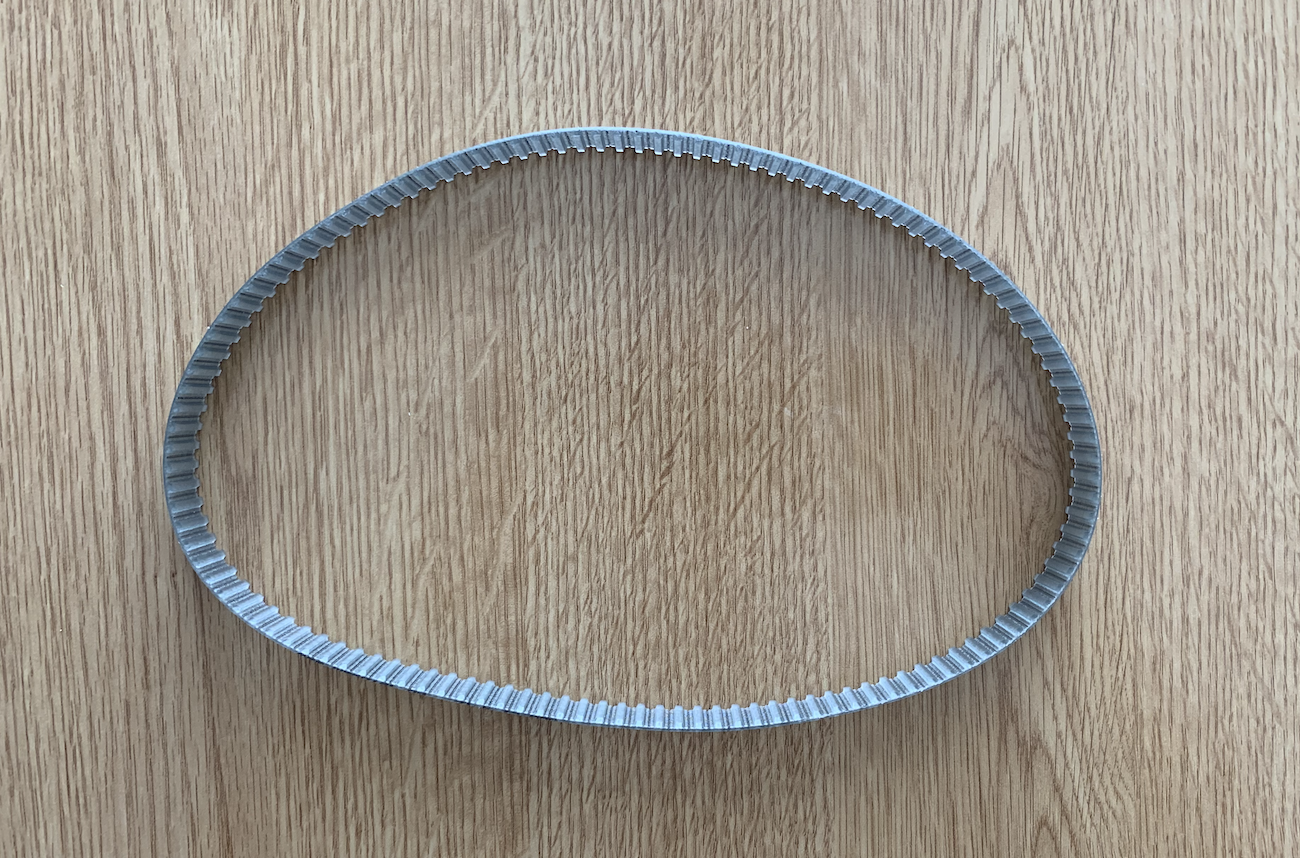
\includegraphics[width=1\textwidth]{img/Gerät Aufbau/Zahnriemen naked.png}
  \centering
  \caption{Zahnriemen}
  \label{fig:Zahnriemen}
\end{figure}

Typ: T5\\

Anzahl Zähne:\\

Länge: \\

Breite: 16 mm
